\documentclass[11pt]{article}

\usepackage[margin=1in, headheight=14pt]{geometry}
\usepackage{amsmath,amssymb,bm,mathtools}
\usepackage{graphicx}
\usepackage{booktabs}
\usepackage{array}
\usepackage{xcolor}
\usepackage{hyperref}
\usepackage{fancyhdr}
\usepackage{lastpage}

\graphicspath{{figures/}}

\pagestyle{fancy}
\fancyhf{}
\lhead{Topology and ICL}
\chead{first-order CRNs}
\rhead{research note}
\cfoot{\thepage}
\renewcommand{\headrulewidth}{0.4pt}

\newcommand{\R}{\mathbb R}
\newcommand{\T}{\mathcal T}
\newcommand{\M}{\mathcal M}
\newcommand{\E}{\mathbb E}
\newcommand{\Cbar}{\bar C}
\newcommand{\drel}{d_{\rm rel}}
\newcommand{\gstar}{\gamma^\ast}

\begin{document}

\thispagestyle{empty}

\noindent
\begin{minipage}[t]{0.60\textwidth}
\raggedright
\textbf{Topology as a Computational Basis for ICL in First-Order CRNs}\\
A concise account of the theory, experiments, audit, and current evidence
\end{minipage}%
\begin{minipage}[t]{0.40\textwidth}
\raggedleft
Topology worktree: \texttt{topology}\\
Evidence source commit: \texttt{ba0e1a69}\\
May 8, 2026
\end{minipage}

\vspace{0.5em}
\noindent\rule{\textwidth}{0.4pt}
\vspace{1.0em}

\noindent\textbf{Summary.}
For first-order CRNs with exponential input-dependent rates, topology is not just a container for trainable parameters. It determines the rooted-spanning-tree sums through which edge projections enter the steady state. The computational basis is therefore not the set of edge vectors $\{K_e\}$, but the set of tree-sum vectors
\[
\boxed{\;\Theta_T=\sum_{e\in T}K_e,\qquad T\in\T_r(G),\ r\in V.\;}
\]
The experiments support the scoped statement that, in the tested fixed-count regimes, topology-associated structural and functional variables explain residual novel-class ICL variation that raw trainable count does not explain. They do not yet give a universal scalar topology law.

\vspace{0.6em}
\noindent\textbf{Scope.}
Everything below is about first-order CRNs with exponential rate encoding. The matrix-tree theorem makes this case exact. Autocatalytic and WTA CRNs need separate topology theories.

\vspace{1em}
\noindent\rule{\textwidth}{0.4pt}
\vspace{1em}

%%%%%%%%%%%%%%%%%%%%%%%%%%%%%%%%%%%%%%%%%%%%%%%%%%%%%%%%%%%%%%%%%%%%%%%%%%%%%%%
\noindent\textbf{[1] The starting question}
%%%%%%%%%%%%%%%%%%%%%%%%%%%%%%%%%%%%%%%%%%%%%%%%%%%%%%%%%%%%%%%%%%%%%%%%%%%%%%%

\vspace{0.5em}
\noindent The original CRN-ICL paper showed that a chemical network can do in-context learning without transformer attention. The input is a context/query vector
\[
z=(z_1,\ldots,z_{N_c},z_q),\qquad z_i\in\R^D,
\]
and the target is the context position whose item matches the query. The true metric is novel-class ICL accuracy, not training accuracy or ordinary validation accuracy.

\vspace{0.5em}
\noindent The paper's mechanism was subspace projection. For each context position $i$, define a comparison region
\[
\M_i=\{z:z_i\sim z_q\}.
\]
ICL succeeds when inputs from different comparison branches produce steady states that the decoder separates.

\vspace{0.5em}
\noindent The original degree-count story was broadly right:
\[
n_{\rm req}=2N_c(N_c+1)D,
\qquad
n_g=N_n(N_n-1)(N_c+1)D
\]
for fully connected first-order CRNs. But this count does not say where the degrees of freedom sit. The topology question was therefore
\[
\boxed{\text{At fixed count, does the reaction/input topology change ICL?}}
\]

\vspace{1em}
\noindent\rule{\textwidth}{0.4pt}
\vspace{1em}

%%%%%%%%%%%%%%%%%%%%%%%%%%%%%%%%%%%%%%%%%%%%%%%%%%%%%%%%%%%%%%%%%%%%%%%%%%%%%%%
\noindent\textbf{[2] The exact first-order object}
%%%%%%%%%%%%%%%%%%%%%%%%%%%%%%%%%%%%%%%%%%%%%%%%%%%%%%%%%%%%%%%%%%%%%%%%%%%%%%%

\vspace{0.5em}
\noindent Let $G=(V,E)$ be a strongly connected directed first-order reaction graph. For edge $e:u\to v$, use exponential rate encoding
\[
k_e(z)=\exp(b_e+K_e^\top z).
\]
The first-order steady state is controlled exactly by the matrix-tree theorem:
\[
\Cbar_r(z)=\frac{\tau_r(z)}{\sum_s\tau_s(z)},
\qquad
\tau_r(z)=\sum_{T\in\T_r(G)}\prod_{e\in T}k_e(z).
\]
Substitute the exponential form:
\[
\prod_{e\in T}k_e(z)
=
\exp\left(\sum_{e\in T}b_e+\left(\sum_{e\in T}K_e\right)^\top z\right).
\]
Set
\[
\beta_T=\sum_{e\in T}b_e,
\qquad
\Theta_T=\sum_{e\in T}K_e.
\]
Then
\[
\boxed{\;\tau_r(z)=\sum_{T\in\T_r(G)}\exp(\beta_T+\Theta_T^\top z).\;}
\]

\vspace{0.5em}
\noindent This is the key point. A first-order CRN does not read out isolated edge projections $K_e^\top z$. It reads out log-sum-exp combinations of rooted-tree projections $\Theta_T^\top z$.

\begin{figure}[h]
\centering
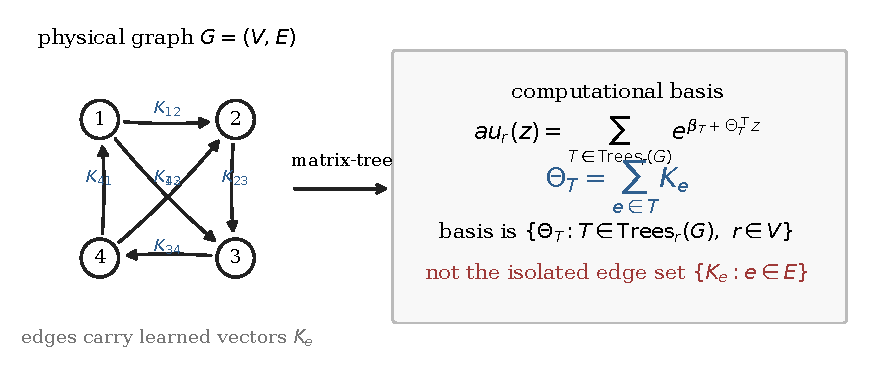
\includegraphics[width=0.95\textwidth]{fig_tree_sum_basis.pdf}
\caption{Topology changes the projection basis. Edge vectors $K_e$ are learned locally, but the steady state uses rooted tree-sum projections $\Theta_T$.}
\end{figure}

\vspace{1em}
\noindent\rule{\textwidth}{0.4pt}
\vspace{1em}

%%%%%%%%%%%%%%%%%%%%%%%%%%%%%%%%%%%%%%%%%%%%%%%%%%%%%%%%%%%%%%%%%%%%%%%%%%%%%%%
\noindent\textbf{[3] What topology changes}
%%%%%%%%%%%%%%%%%%%%%%%%%%%%%%%%%%%%%%%%%%%%%%%%%%%%%%%%%%%%%%%%%%%%%%%%%%%%%%%

\vspace{0.5em}
\noindent Stack tree incidences as row vectors $s_T\in\{0,1\}^m$. Then
\[
\Theta_T=K^\top s_T.
\]
Since concentrations are normalized, common shifts of all tree scores cancel. The more relevant structural object is the tree-difference matrix
\[
D_G=
\begin{bmatrix}
s_{T_1}-s_{T_0}\\
s_{T_2}-s_{T_0}\\
\vdots
\end{bmatrix}.
\]
A first count of relative projection capacity is
\[
\drel(G)=p\,\operatorname{rank}(D_G),
\qquad p=(N_c+1)D.
\]
With an input mask $\Omega_{e\alpha}$, the capacity must be input-aware:
\[
\boxed{\;\drel(G,\Omega)=\sum_{\alpha=1}^{p}\operatorname{rank}\big(D_G\operatorname{diag}(\Omega_{\cdot\alpha})\big).\;}
\]

\vspace{0.5em}
\noindent But this is still only a rank proxy. ICL asks a sharper question:
\[
\boxed{\text{Can the allowed tree-sum directions separate the comparison branches?}}
\]
The capacity object should be closer to
\[
\gstar(G,\Omega)=\max_{K,B}\min_{z\in\mathcal B}
\left[q_{\ell^\ast(z)}(z)-\max_{\ell\neq \ell^\ast(z)}q_\ell(z)\right]
\]
under norm constraints. In the tropical limit,
\[
\log\tau_r(z)\approx\max_{T\in\T_r(G)}(\beta_T+\Theta_T^\top z),
\]
so the theory becomes a rooted-tree-polytope normal-fan coverage problem.

\vspace{0.5em}
\noindent The hierarchy that emerged is therefore
\[
\begin{aligned}
\text{raw count}
&<\text{relative tree rank}
<\text{masked tree geometry}\\
&<\text{branch-margin/tree-polytope geometry}
<\text{trained organization}
<\text{causal dependence}.
\end{aligned}
\]

\vspace{1em}
\noindent\rule{\textwidth}{0.4pt}
\vspace{1em}

%%%%%%%%%%%%%%%%%%%%%%%%%%%%%%%%%%%%%%%%%%%%%%%%%%%%%%%%%%%%%%%%%%%%%%%%%%%%%%%
\noindent\textbf{[4] What was built and audited}
%%%%%%%%%%%%%%%%%%%%%%%%%%%%%%%%%%%%%%%%%%%%%%%%%%%%%%%%%%%%%%%%%%%%%%%%%%%%%%%

\vspace{0.5em}
\noindent The worktree now contains code and reports for arbitrary first-order directed topologies, input masks, tree metrics, branch-capacity probes, post-training tree diagnostics, ablations, motif extraction, and statistic-preserving causal scrambles.

\vspace{0.5em}
\noindent The audit report \texttt{ICL/results/next\_phase\_stats/topology\_goal\_completion\_audit.md} maps the goal to concrete artifacts. It records that the verifier passed for committed artifacts, that hard regimes have full result/model/mechanism/causal follow-ups, and that all headline claims are scoped to \texttt{test\_novel\_classes}. The audit also marks the branch-margin theory as partial by design: proxies exist, but there is not yet a final theorem.

\vspace{0.5em}
\noindent The main source reports used here are:
\begin{center}
\small
\begin{tabular}{p{0.48\textwidth}p{0.40\textwidth}}
\texttt{topology\_icl\_complete\_explanation.md} & full narrative explanation\\
\texttt{next\_phase\_evidence\_report.md/json} & fixed-count, motif, causal summaries\\
\texttt{mechanism\_isolation\_evidence.csv} & controlled mechanism contrasts\\
\texttt{stat\_preserving\_causal\_stratified} & stratified causal scrambles\\
\texttt{degree\_rewire\_normal\_fan\_...} & exact-degree normal-fan pilot
\end{tabular}
\end{center}

\vspace{1em}
\noindent\rule{\textwidth}{0.4pt}
\vspace{1em}

%%%%%%%%%%%%%%%%%%%%%%%%%%%%%%%%%%%%%%%%%%%%%%%%%%%%%%%%%%%%%%%%%%%%%%%%%%%%%%%
\noindent\textbf{[5] Fixed-count structural evidence}
%%%%%%%%%%%%%%%%%%%%%%%%%%%%%%%%%%%%%%%%%%%%%%%%%%%%%%%%%%%%%%%%%%%%%%%%%%%%%%%

\vspace{0.5em}
\noindent The original controlled regime fixed
\[
N_n=6,
\qquad m=20,
\qquad \text{input-coupled count}=200.
\]
It used three physical backbones, 16 selected masks/topologies per backbone, five training seeds each, 240 total runs, and 48 topology/mask groups.

\vspace{0.5em}
\noindent At group level, with target equal to mean novel-class ICL accuracy, the leave-one-out values were
\begin{center}
\begin{tabular}{l c p{0.45\textwidth}}
\toprule
model & group LOO $R^2$ & interpretation\\
\midrule
raw count & $-0.043$ & no explanatory power at fixed count\\
raw count+$\drel$ & $0.145$ & relative rank helps\\
masked tree geometry & $0.189$ & input-aware geometry helps\\
tree geometry & $0.409$ & strongest structural summary here\\
\bottomrule
\end{tabular}
\end{center}
The corresponding hard $N_n=5,m=12,N_c=3,D=2$ regime showed a different but still positive pattern: raw count and $\drel$ alone were both $-0.190$, tree geometry was $0.324$, and masked tree geometry was $0.447$.

\begin{figure}[h]
\centering
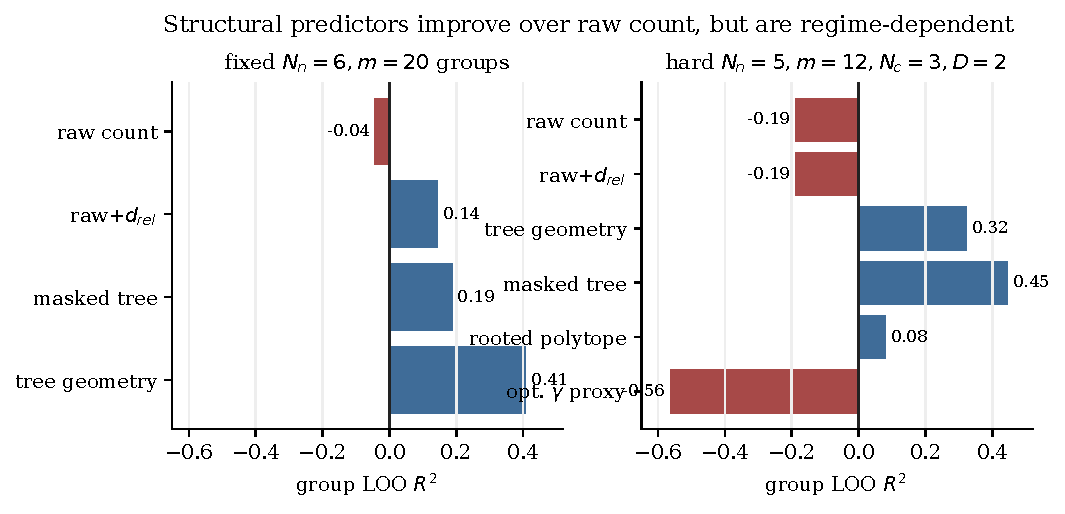
\includegraphics[width=0.98\textwidth]{fig_structural_predictors.pdf}
\caption{Structural predictors in two fixed-count regimes. Raw count is uninformative once fixed. Tree geometry and masked tree geometry explain residual group-level variation, but the best predictor depends on regime.}
\end{figure}

\vspace{0.5em}
\noindent The safe conclusion is not that $\drel$ is the law. It is that topology-associated variables explain residual ICL variation that raw count cannot explain in the tested regimes.

\vspace{1em}
\noindent\rule{\textwidth}{0.4pt}
\vspace{1em}

%%%%%%%%%%%%%%%%%%%%%%%%%%%%%%%%%%%%%%%%%%%%%%%%%%%%%%%%%%%%%%%%%%%%%%%%%%%%%%%
\noindent\textbf{[6] Why input masks matter}
%%%%%%%%%%%%%%%%%%%%%%%%%%%%%%%%%%%%%%%%%%%%%%%%%%%%%%%%%%%%%%%%%%%%%%%%%%%%%%%

\vspace{0.5em}
\noindent Physical topology and input-encoding topology are distinct. The physical graph fixes the rooted trees:
\[
G_{\rm phys}\mapsto \T_r(G).
\]
The input mask fixes which coordinates can enter which edge vectors:
\[
\Omega_{e\alpha}=0\quad\Rightarrow\quad K_{e\alpha}=0.
\]
The real capacity object is therefore $\gstar(G,\Omega)$, not only $\gstar(G)$.

\vspace{0.5em}
\noindent The mechanism-isolation file shows fixed-graph, fixed-count, fixed-$\drel$ cases where masks still change ICL. On the fixed random physical graph, changing edge-load structure gave $+6.96$ mean ICL points, while changing coordinate-load heterogeneity gave $-16.48$ mean ICL points. On the fixed cycle graph, the corresponding deltas were $-6.32$ and $+2.12$ points; on the fixed hub graph they were $+3.44$ and $-1.52$ points. The sign is not universal, but the effect exists.

\begin{figure}[h]
\centering
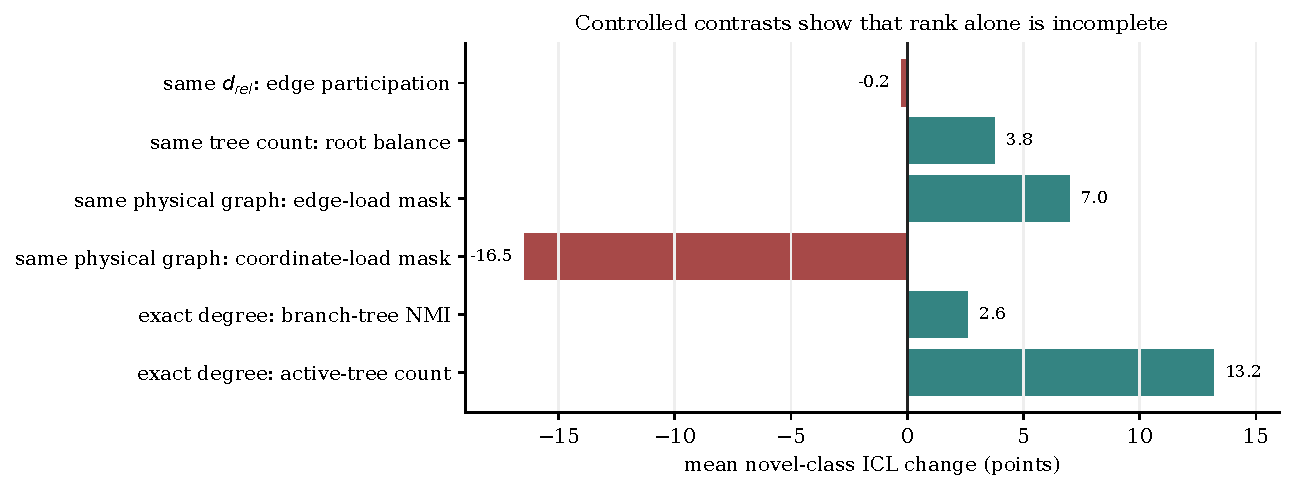
\includegraphics[width=0.95\textwidth]{fig_mechanism_contrasts.pdf}
\caption{Controlled contrasts. Some coarse structural metrics are not monotone drivers, and fixed-graph input masks can still change ICL. This is why $\drel$ alone is incomplete.}
\end{figure}

\vspace{1em}
\noindent\rule{\textwidth}{0.4pt}
\vspace{1em}

%%%%%%%%%%%%%%%%%%%%%%%%%%%%%%%%%%%%%%%%%%%%%%%%%%%%%%%%%%%%%%%%%%%%%%%%%%%%%%%
\noindent\textbf{[7] Post-training mechanism evidence}
%%%%%%%%%%%%%%%%%%%%%%%%%%%%%%%%%%%%%%%%%%%%%%%%%%%%%%%%%%%%%%%%%%%%%%%%%%%%%%%

\vspace{0.5em}
\noindent Pre-training topology asks what the graph could use. Post-training diagnostics ask what the trained model did use. The strongest diagnostic class was projection/root/tree organization around comparison branches. Projection-alignment summaries gave
\[
\begin{aligned}
R^2_{\rm LOO}&=0.740 &&\text{at run level},\\
R^2_{\rm LOO}&=0.809 &&\text{at topology-mean level},\\
R^2_{\rm LOO}&=0.599 &&\text{for topology-best seed}.
\end{aligned}
\]

\begin{figure}[h]
\centering
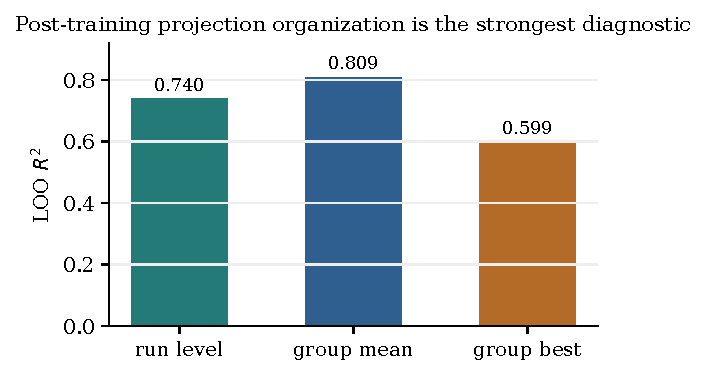
\includegraphics[width=0.62\textwidth]{fig_post_training_alignment.pdf}
\caption{Post-training projection alignment is much more explanatory than coarse pre-training count. This is mechanism evidence, not an independent capacity theorem.}
\end{figure}

\vspace{0.5em}
\noindent This means high-ICL models are not merely high-count systems. They organize the available tree-sum geometry so that comparison branches produce decodable steady states. The active-tree and margin diagnostics are close to the learned mechanism, so they should be read as mechanistic explanations rather than clean pre-training predictors.

\vspace{1em}
\noindent\rule{\textwidth}{0.4pt}
\vspace{1em}

%%%%%%%%%%%%%%%%%%%%%%%%%%%%%%%%%%%%%%%%%%%%%%%%%%%%%%%%%%%%%%%%%%%%%%%%%%%%%%%
\noindent\textbf{[8] Causal scrambles}
%%%%%%%%%%%%%%%%%%%%%%%%%%%%%%%%%%%%%%%%%%%%%%%%%%%%%%%%%%%%%%%%%%%%%%%%%%%%%%%

\vspace{0.5em}
\noindent The causal interventions are the strongest evidence that the learned alignment matters. Two statistic-preserving scrambles were central:
\begin{center}
\begin{tabular}{p{0.32\textwidth}p{0.56\textwidth}}
branch-alignment scramble & preserves graph, root tree counts, $\drel$, and input density\\
projection scramble & also preserves input support and per-edge projection row norms
\end{tabular}
\end{center}
They break branch/projection/tree organization while preserving many coarse statistics.

\vspace{0.5em}
\noindent In the stratified hard-regime pilot, high-ICL runs dropped by about $-96$ points under branch-alignment scrambling and about $-64$ to $-68$ points under projection scrambling. Low and mid runs also collapsed substantially.

\begin{figure}[h]
\centering
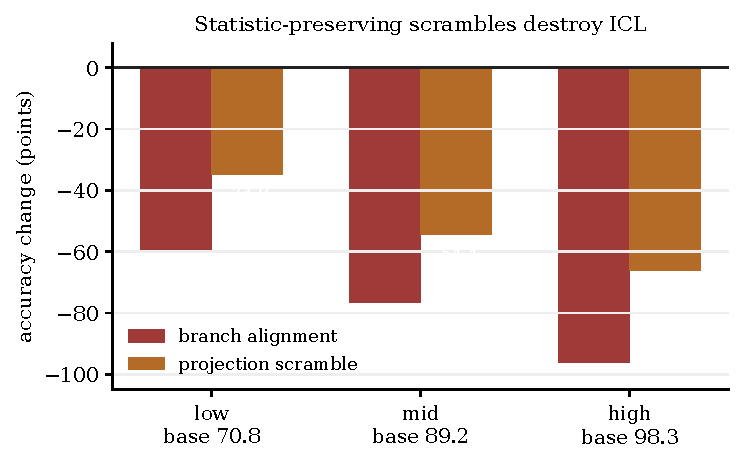
\includegraphics[width=0.72\textwidth]{fig_causal_scrambles.pdf}
\caption{Statistic-preserving scrambles in low, mid, and high baseline buckets. Destroying branch/projection/tree alignment sharply reduces novel-class ICL.}
\end{figure}

\vspace{0.5em}
\noindent This pushes the evidence beyond correlation. It says the trained CRNs rely on the organized relation between input branches, learned edge projections, and root/tree structure.

\vspace{1em}
\noindent\rule{\textwidth}{0.4pt}
\vspace{1em}

%%%%%%%%%%%%%%%%%%%%%%%%%%%%%%%%%%%%%%%%%%%%%%%%%%%%%%%%%%%%%%%%%%%%%%%%%%%%%%%
\noindent\textbf{[9] Hard regimes and the normal-fan pilot}
%%%%%%%%%%%%%%%%%%%%%%%%%%%%%%%%%%%%%%%%%%%%%%%%%%%%%%%%%%%%%%%%%%%%%%%%%%%%%%%

\vspace{0.5em}
\noindent Three hard regimes were added: $n4\_m6\_N3\_D2$, $n5\_m8\_N3\_D2$, and $n5\_m12\_N3\_D2$, each with 60 trained runs plus mechanism and causal follow-ups. The results are mixed in the useful sense. Topology signal depends on regime.

\vspace{0.5em}
\noindent In $n5\_m12\_N3\_D2$, masked tree geometry had LOO $R^2=0.447$ and positive held-out-family performance. In the sparser $n5\_m8\_N3\_D2$ regime, within-sample bootstrap improvements were more positive than held-out-family prediction. This suggests that topology may have sparse, intermediate, and redundant regimes rather than one monotone scalar rule.

\vspace{0.5em}
\noindent The exact-degree normal-fan pilot fixed
\[
N_n=5,
\quad m=12,
\quad N_c=3,
\quad D=2,
\quad \text{in/out degree sequence}=[3,2,2,3,2],
\quad \drel=88.
\]
It varied tree-polytope/normal-fan diagnostics through directed degree-preserving rewires. Only four topology groups were trained, so this is not yet a statistical result. It is a constructive design showing that topology can vary beyond degree sequence and $\drel$.

\begin{figure}[h]
\centering
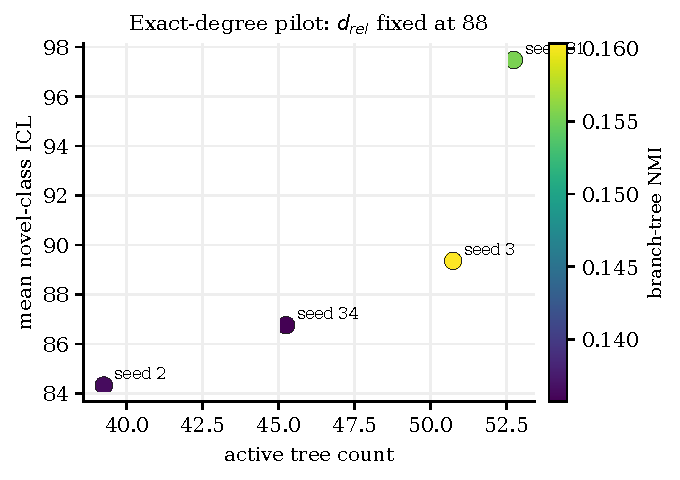
\includegraphics[width=0.62\textwidth]{fig_degree_rewire_pilot.pdf}
\caption{Exact-degree pilot. All points have the same degree sequence and $\drel=88$. Active tree count and branch-tree NMI vary across rewires, and mean ICL varies with them in this small $n=4$ pilot.}
\end{figure}

\vspace{0.5em}
\noindent The descriptive $n=4$ correlations were $r=0.869$ for active-tree count and $r=0.691$ for branch-tree NMI with mean ICL. These numbers are promising design feedback, not proof.

\vspace{1em}
\noindent\rule{\textwidth}{0.4pt}
\vspace{1em}

%%%%%%%%%%%%%%%%%%%%%%%%%%%%%%%%%%%%%%%%%%%%%%%%%%%%%%%%%%%%%%%%%%%%%%%%%%%%%%%
\noindent\textbf{[10] Motifs and matched controls}
%%%%%%%%%%%%%%%%%%%%%%%%%%%%%%%%%%%%%%%%%%%%%%%%%%%%%%%%%%%%%%%%%%%%%%%%%%%%%%%

\vspace{0.5em}
\noindent Essential physical subgraphs retrained better than sparse input masks under the extraction protocol. But matched controls softened the stronger interpretation. Degree-rewired and random strongly connected controls often matched or exceeded the extracted motifs.

\begin{figure}[h]
\centering
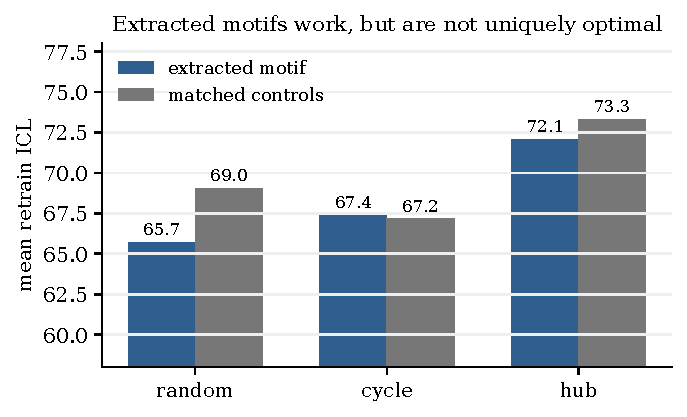
\includegraphics[width=0.68\textwidth]{fig_motif_controls.pdf}
\caption{Extracted physical motifs support ICL, but matched controls are competitive. The evidence supports a family of feasible physical substrates, not one unique motif.}
\end{figure}

\vspace{0.5em}
\noindent The corrected interpretation is:
\[
\boxed{\text{small physical subgraphs can support ICL, but the extracted motifs are not uniquely optimal.}}
\]
This is compatible with the tree-sum view: many different graphs can provide usable branch-covering tree geometry.

\vspace{1em}
\noindent\rule{\textwidth}{0.4pt}
\vspace{1em}

%%%%%%%%%%%%%%%%%%%%%%%%%%%%%%%%%%%%%%%%%%%%%%%%%%%%%%%%%%%%%%%%%%%%%%%%%%%%%%%
\noindent\textbf{[11] The gamma-star attempt}
%%%%%%%%%%%%%%%%%%%%%%%%%%%%%%%%%%%%%%%%%%%%%%%%%%%%%%%%%%%%%%%%%%%%%%%%%%%%%%%

\vspace{0.5em}
\noindent The project implemented $\gstar$-style capacity probes because $\drel$ is too coarse. This was the right theoretical direction, but the current optimized proxy did not outperform tree geometry. In the hard $n5\_m12\_N3\_D2$ regression, optimized $\gamma$ capacity had LOO $R^2=-0.564$, while tree geometry had $0.324$ and masked tree geometry had $0.447$.

\vspace{0.5em}
\noindent This is an informative failure. The surrogate likely optimizes smooth average behavior more than the true worst-branch margin. ICL is closer to a worst-branch problem:
\[
\max_{K,B}\min_{b\in\mathcal B}\operatorname{margin}_b(K,B;G,\Omega).
\]
A good capacity theory should target low-percentile or worst-branch separation under norm constraints.

\vspace{1em}
\noindent\rule{\textwidth}{0.4pt}
\vspace{1em}

%%%%%%%%%%%%%%%%%%%%%%%%%%%%%%%%%%%%%%%%%%%%%%%%%%%%%%%%%%%%%%%%%%%%%%%%%%%%%%%
\noindent\textbf{[12] What has been achieved}
%%%%%%%%%%%%%%%%%%%%%%%%%%%%%%%%%%%%%%%%%%%%%%%%%%%%%%%%%%%%%%%%%%%%%%%%%%%%%%%

\vspace{0.5em}
\noindent Before this direction, the paper had:
\[
\text{CRNs can do ICL by subspace projection, and raw learned degrees of freedom are important.}
\]
After this direction, the first-order story is sharper:
\begin{center}
\fbox{\begin{minipage}{0.86\textwidth}
raw degrees are useful only insofar as topology and masks turn them into relative tree-sum projections that cover comparison branches.
\end{minipage}}
\end{center}

\vspace{0.5em}
\noindent The concrete accomplishments are:
\begin{center}
\small
\begin{tabular}{p{0.25\textwidth}p{0.64\textwidth}}
\toprule
Layer & What was established\\
\midrule
Theory & The exact first-order computational basis is the rooted tree-sum basis $\{\Theta_T\}$, not the isolated edge basis $\{K_e\}$.\\
Structural evidence & Fixed-count regimes show residual ICL variation explained by tree and masked-tree geometry beyond raw count.\\
Input topology & Fixed physical graph/count/$\drel$ masks can still differ sharply, so the object is $\gstar(G,\Omega)$.\\
Mechanism & Successful trained models organize projection/root/tree features around comparison branches.\\
Causality & Statistic-preserving scrambles that break alignment sharply reduce ICL.\\
Limits & $\drel$ is not a capacity law; current $\gamma$ probes are not final; motifs are not unique; nonlinear CRNs are out of scope.\\
\bottomrule
\end{tabular}
\end{center}

\vspace{0.5em}
\noindent The most defensible statement is:
\begin{center}
\fbox{\begin{minipage}{0.86\textwidth}
In the tested first-order fixed-count regimes, topology-associated structural and functional variables explain residual novel-class ICL variation that raw trainable count does not explain. The strongest mechanism evidence is that trained models depend on branch/projection/tree alignment.
\end{minipage}}
\end{center}

\vspace{1em}
\noindent\rule{\textwidth}{0.4pt}
\vspace{1em}

%%%%%%%%%%%%%%%%%%%%%%%%%%%%%%%%%%%%%%%%%%%%%%%%%%%%%%%%%%%%%%%%%%%%%%%%%%%%%%%
\noindent\textbf{[13] What should come next}
%%%%%%%%%%%%%%%%%%%%%%%%%%%%%%%%%%%%%%%%%%%%%%%%%%%%%%%%%%%%%%%%%%%%%%%%%%%%%%%

\vspace{0.5em}
\noindent The next phase should not be a loose sweep. It should scale the exact-degree/normal-fan design:
\[
\begin{gathered}
\text{fix }N_n,m,N_c,D,\text{ input count, degree sequence, and }\drel,\\
\text{vary tree-polytope and normal-fan diagnostics, then train enough groups for grouped inference.}
\end{gathered}
\]
Then compare raw count, $\drel$, masked tree geometry, normal-fan diagnostics, and an improved worst-branch $\gstar(G,\Omega)$ probe.

\vspace{0.5em}
\noindent The theoretical target is:
\begin{center}
\fbox{\begin{minipage}{0.86\textwidth}
derive a norm-constrained tree-polytope branch-margin capacity that predicts whether $(G,\Omega)$ can cover ICL branches.
\end{minipage}}
\end{center}
That would turn the current empirical and mechanistic evidence into a true first-order topology theory.

\end{document}
